\documentclass{beamer}

\usetheme{Padova}
\usepackage[absolute,overlay]{textpos}
\usepackage{float}
\usepackage[utf8]{inputenc}

\subtitle{Dipartimento di Matematica "Tullio Levi-Civita"\\
Corso di Laurea in Informatica}
\title{Implementazione di una interfaccia SAPI 5 mediante i sistemi di sintesi vocale MaryTTS e Speect }
\author{Laureando: Cristian Andrighetto\\
		Relatore: Paolo Baldan}
\date{20 Luglio 2017}


\begin{document}

	\maketitle

	\section{L'azienda}

	\begin{frame}{L'azienda}

		\begin{figure}[H]
			\centering
			
\includegraphics{images/logo-mivoq.png}
		\end{figure}
	
		\begin{itemize}
			\item start-up
			\item sede a Padova ospitata dall'Istituto di Scienze e Tecnologie della Cognizione (ISTC) che fa parte del CNR
			\item si occupa di tecnologie vocali
			\item personalizzazione della voce
			
		\end{itemize}
	\end{frame}

	\section{Sintesi Vocale}
	
	\begin{frame}{Sintesi Vocale}
		\begin{textblock*}{5cm}(1cm,2cm) % {block width} (coords)
			
\includegraphics[width=5cm]{images/marylogo}
		\end{textblock*}
		\begin{textblock*}{5cm}(7cm,2cm) % {block width} (coords)
			
\includegraphics[width=5cm]{images/speect_logo_full}
		\end{textblock*}
	    \vspace{50pt}
		\textbf{Progetti in corso di sviluppo}
		\begin{itemize}
			\item piattaforma \textbf{FATTS} che integra \textbf{MaryTTS}
			\item engine TTS \textbf{Speect}
		\end{itemize}
		\vspace{10pt}
		\textbf{Obiettivo dell'azienda}
		\begin{itemize}
			\item abbandonare \textbf{MaryTTS} per adottare \textbf{Speect} 
		\end{itemize}
	\end{frame}


	\section{Problema affrontato}

	\begin{frame}{Problema affrontato}
		Integrazione degli \textbf{engine Text-To-Speech} con \textbf{Microsoft Windows} attraverso l'interfaccia \textbf{SAPI 5}
		\begin{itemize}
		\item \textbf{rendere funzionanti} gli engine TTS con Microsoft Windows
		\item \textbf{studiare} l'interfaccia SAPI 5 per trovare la soluzione migliore
		\item rendere disponibili la maggior parte delle funzionalità messe a disposizione dagli engine TTS all'utente
		\end{itemize}
		\vspace{10pt}
		Aggiungere funzionalità a \textbf{Speect}
		\begin{itemize}
			\item regolazione \textbf{tonalità} voce
			\item regolazione \textbf{velocità} voce
		\end{itemize}
	\end{frame}

	\section{Soluzione}
	
	\begin{frame}{Soluzione}
		Per \textbf{MaryTTS}
		\begin{itemize}
			\item implementazione dell'interfaccia SAPI 5
			\item componente per la comunicazione con MaryTTS
		\end{itemize}
		Per \textbf{Speect}
		\begin{itemize}
			\item implementazione dell'interfaccia SAPI 5
			\item nuova classe per abilitare la \textbf{serializzazione} di uno stream audio in un buffer
			\item nuovi metodi per controllare la \textbf{velocità} e \textbf{tonalità} della voce
		\end{itemize}
	\end{frame}

	\section{Specifica SAPI 5}
	
	\begin{frame}{Specifica SAPI 5}
		\begin{figure}[H]
			\centering
			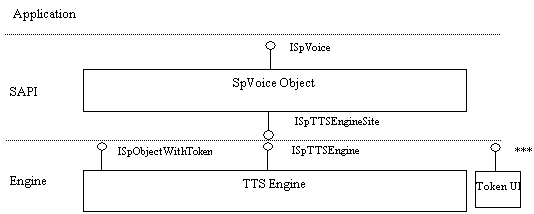
\includegraphics[width=\textwidth]{images/specifica-sapi5}
		\end{figure}
	\end{frame}

	\section{Architettura per MaryTTS}
	
	\begin{frame}{Architettura per MaryTTS}
		\begin{figure}[H]
			\centering
			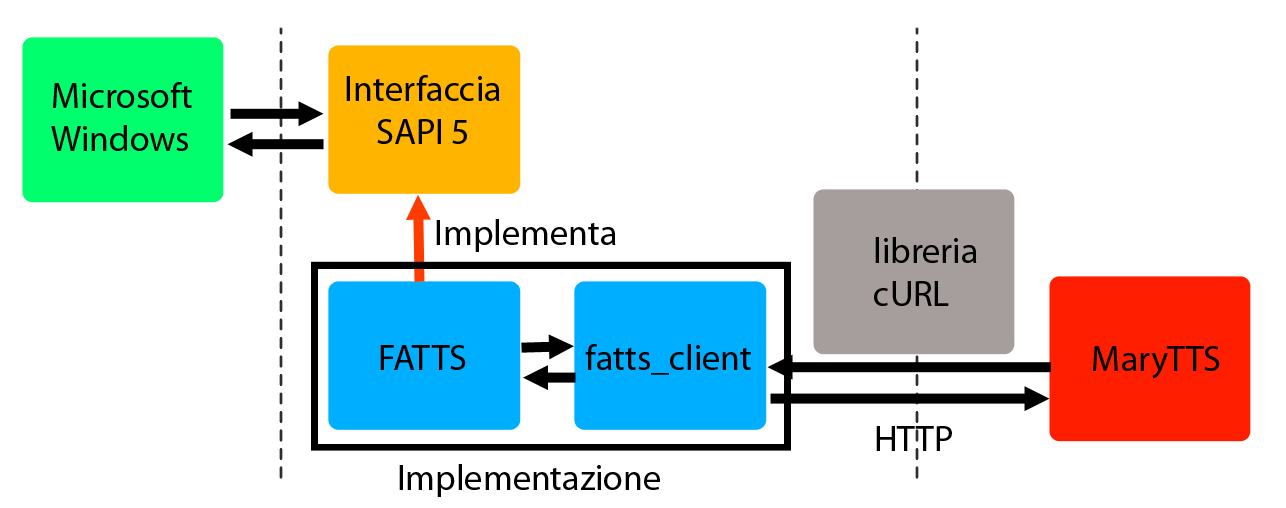
\includegraphics[width=\textwidth]{images/FATTS-sapi5.png}
		\end{figure}
	\end{frame}

	\section{Architettura per Speect}
	
	\begin{frame}{Archittetura per Speect}
		\begin{figure}[H]
			\centering
			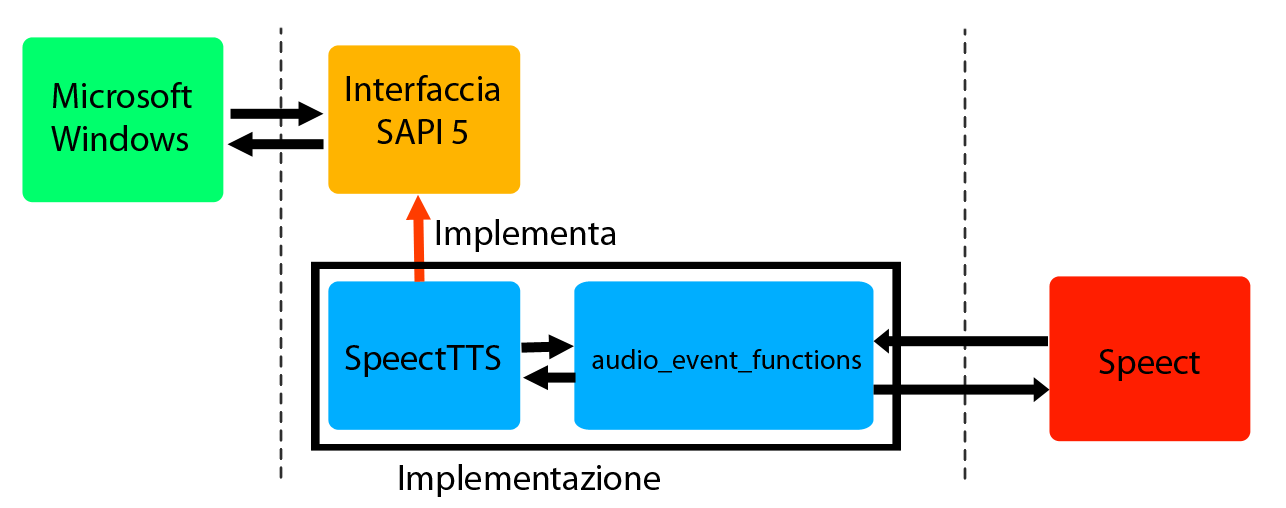
\includegraphics[width=\textwidth]{images/SpeectTTS-sapi5.png}
		\end{figure}
	\end{frame}

	\section{Tecnologie Utilizzate}
	
	\begin{frame}{Tecnologie Utilizzate}
		\begin{textblock*}{5cm}(1.5cm,1.5cm) % {block width} (coords)
			
\includegraphics[width=4cm]{images/windows-logo}
		\end{textblock*}
		\begin{textblock*}{5cm}(1cm,3.2cm) % {block width} (coords)
			
\includegraphics[width=3cm]{images/visualstudio-logo}
		\end{textblock*}
		\begin{textblock*}{5cm}(4.7cm,3.1cm) % {block width} (coords)
			
\includegraphics[width=2cm]{images/c_cplusplus}
		\end{textblock*}
		\begin{textblock*}{4cm}(1.5cm,4.5cm) % {block width} (coords)
			Microsoft Speech API 5
		\end{textblock*}
		\begin{textblock*}{5cm}(2cm,5.5cm) % {block width} (coords)
			
\includegraphics[width=2cm]{images/git-logo}
		\end{textblock*}
		\begin{textblock*}{5cm}(0.5cm,6.5cm) % {block width} (coords)
			
\includegraphics[width=3cm]{images/github-logo}
		\end{textblock*}
		\begin{textblock*}{5cm}(3.5cm,6.5cm) % {block width} (coords)
			
\includegraphics[width=1.5cm]{images/gitlab}
		\end{textblock*}
		\begin{textblock*}{5cm}(7.3cm,5.3cm) % {block width} (coords)
			
\includegraphics[width=2.5cm]{images/curl_logo}
		\end{textblock*}
		\begin{textblock*}{5cm}(8cm,2.5cm) % {block width} (coords)
			TTS Application
		\end{textblock*}
		\begin{textblock*}{5cm}(8.2cm,3cm) % {block width} (coords)
			
\includegraphics[width=2.5cm]{images/balabolka}
		\end{textblock*}
		\begin{textblock*}{5cm}(8cm,6.5cm) % {block width} (coords)
			
\includegraphics[width=4cm]{images/marylogo}
		\end{textblock*}
		\begin{textblock*}{5cm}(6.5cm,7.5cm) % {block width} (coords)
			
\includegraphics[width=4cm]{images/speect_logo_full}
		\end{textblock*}
		\begin{textblock*}{5cm}(11.3cm,3cm) % {block width} (coords)
			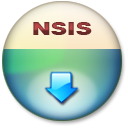
\includegraphics[width=1.2cm]{images/NSIS-logo}
		\end{textblock*}
		
\end{frame}

\section{Prodotto Finale}
\begin{frame}{Prodotto Finale}
	\begin{itemize}
		\item Libreria a caricamento dinamico (\textbf{DLL}) per ogni implementazione
		\item Installazione automatica tramite pacchetto \textbf{NSIS}
	\end{itemize}
	\begin{figure}[H]
		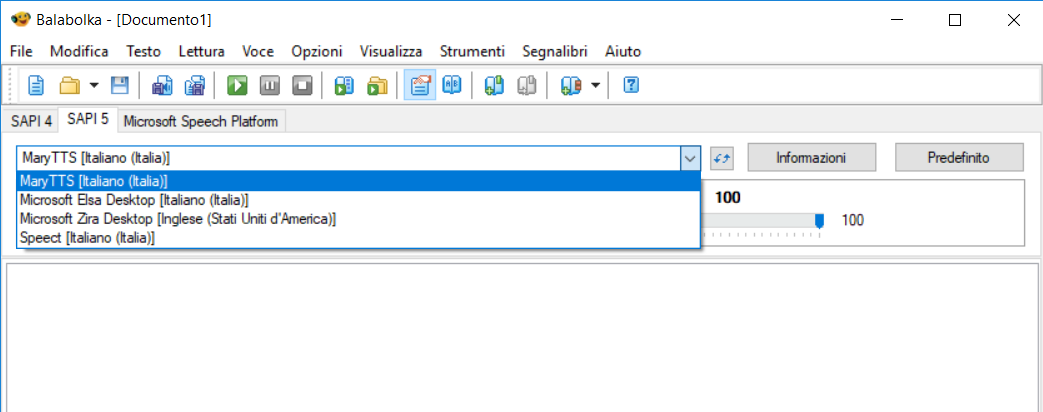
\includegraphics[width=\textwidth]{images/prodotto-finale}
	\end{figure}
\end{frame}

\section{Prodotto Finale}
\begin{frame}{Prodotto Finale}
	\begin{itemize}
		\item Controllo dei parametri della voce  (\textbf{tonalità}, \textbf{velocità} e 
	    \textbf{volume})
		\item Supportati ora anche da Speect 
	\end{itemize}
	\begin{figure}[H]
		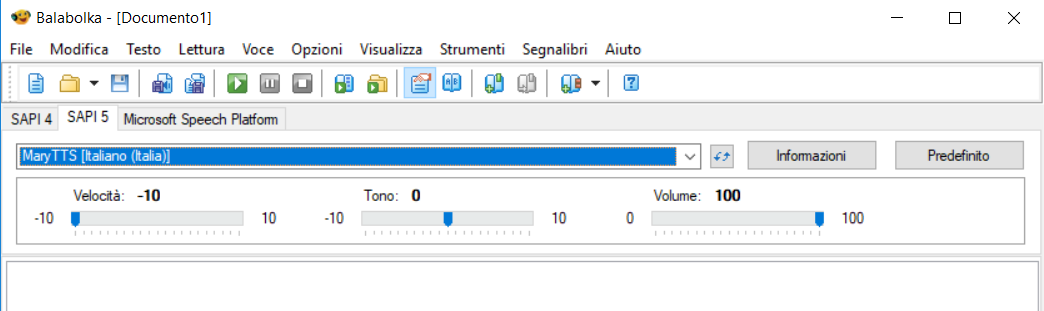
\includegraphics[width=\textwidth]{images/prodotto-finale-2}
	\end{figure}
\end{frame}

\section{Prodotto Finale}
\begin{frame}{Prodotto Finale}
	\begin{itemize}
	 \item Controllo di un avatar 
	 \item Evidenziare il testo riprodotto
	\end{itemize}
	\begin{figure}[H]
		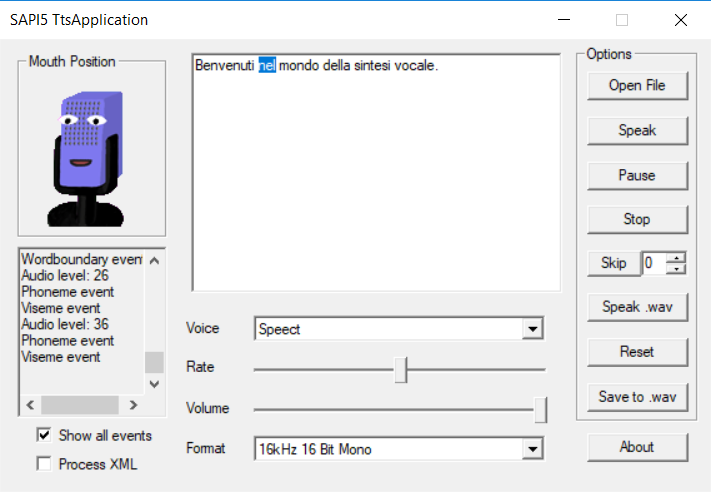
\includegraphics[height=6cm]{images/prodotto-finale-3}
	\end{figure}
	\begin{textblock*}{1cm}(1cm,6.5cm) % {block width} (coords)
		Eventi SAPI
	\end{textblock*}
	
\end{frame}

\section{Considerazioni finali}
\begin{frame}{Considerazioni finali}
	\textbf{Risultato}
	\begin{itemize}
		\item tutti gli obiettivi \textbf{obbligatori} sono stati soddisfatti
		\item nuovo ramo di sviluppo per l'azienda
		\item entrambi gli engine TTS sono compatibili con i sistemi operativi \textbf{Microsoft Windows} e \textbf{GNU/Linux}
	\end{itemize}
	\vspace{10pt}
	\textbf{Problemi riscontrati}
	\begin{itemize}
		\item compilazione problematica dell'engine Speect 
	\end{itemize}
    \vspace{10pt}
	\textbf{Sviluppi futuri}
	\begin{itemize}
		\item integrazione completa con il sistema Microsoft Windows
		\item utilizzare applicazioni sfruttando la propria voce
	\end{itemize}
\end{frame}

	

	


\end{document}
